% ====================================================================
%+
% SECTION:
%    grb.tex
%
% CHAPTER:
%    transients.tex
%
% ELEVATOR PITCH:
%-
% ====================================================================

\section{Gamma-Ray Burst Afterglows}
\def\secname{grbs}\label{sec:\secname}

\credit{ebellm}

Gamma-ray bursts (GRBs) are relativistic explosions typically classified
by the temporal duration of their initial gamma-ray emission: Long GRBs,
that mark the endpoint of the lives of some massive stars, and short
GRBs, believed to originate from the merger of binary neutron stars. GRB
emission is known to be beamed: the initial prompt gamma-ray emission is
seen only for observers looking at the jet axis. The longer-wavelength
X-ray, optical, and radio afterglow may be seen both by on- and off-axis
observers.  The latter case is known as an orphan afterglow, due to the
absence of gamma-ray emission. On- and off-axis afterglows are predicted
to have different temporal signatures in the optical: On-axis events
decay as a power-law until a jet break, while off-axis events should be
fainter and show an initial rise (Figure \ref{fig:afterglow_lcs}).
Despite systematic searches, no convincing orphan afterglow candidates
have yet been discovered, limiting our knowledge of the beaming fraction
of GRBs and hence their true rates. Well-sampled orphan afterglow
lightcurves would also permit study of the GRB jet structure.

\begin{figure}[hbt]
\centerline{
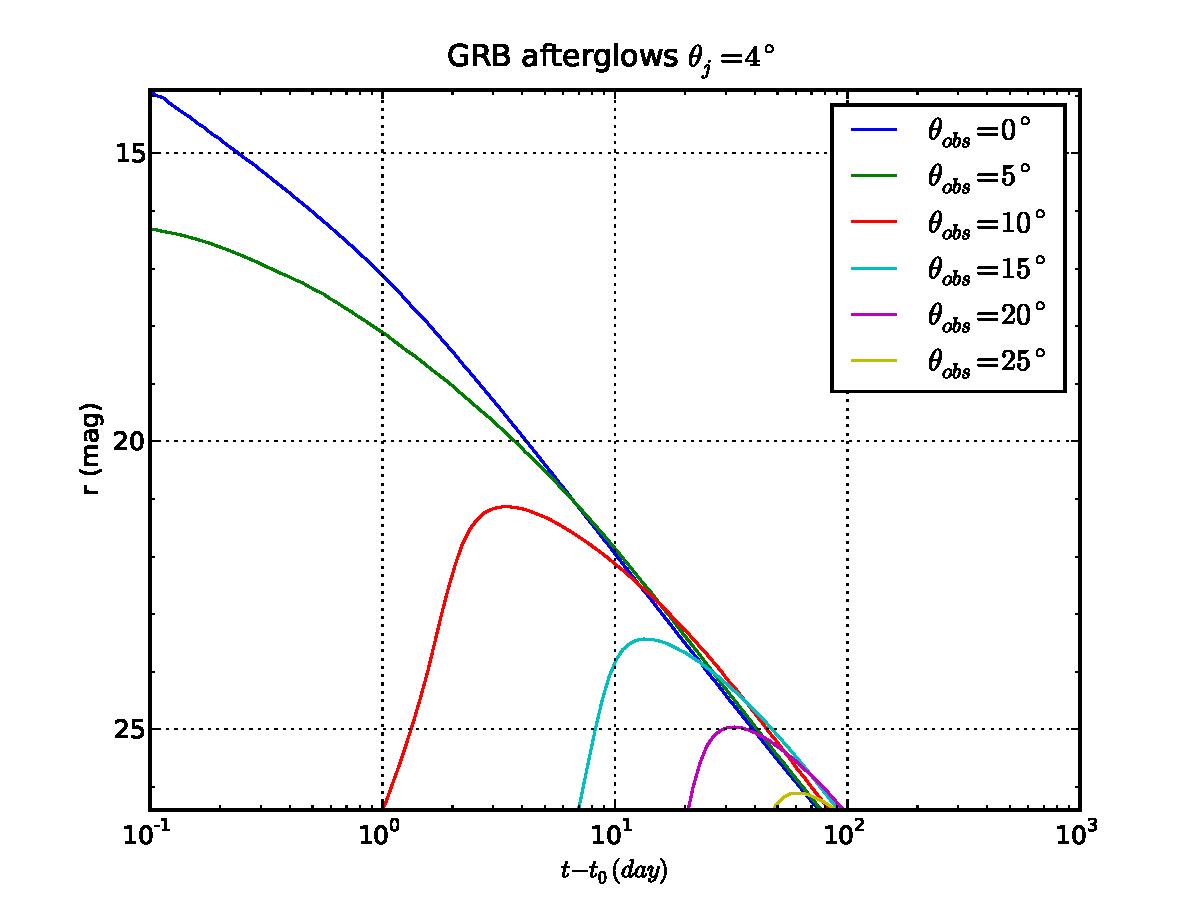
\includegraphics[width=0.6\textwidth]{figs/transients/predicted_afterglow_lcs_mag.pdf}
}
\caption{ Predicted light curves of GRB afterglows by off-axis angle
with respect to the jet axis $\theta_{\rm obs}$ \citep[Figure
8.8,][]{2009arXiv0912.0201L}. The forward shock model is derived from
\citet{2002ApJ...576..120T} and assumes a jet half opening angle
$\theta_j = 4^\circ$, the isotropic equivalent energy of $E_{\rm iso} =
5\times10^{53} \rm erg$, ambient medium density $n = 1$ g cm$^{-3}$, and
the slope of the electron energy distribution $\rm p = 2.1$. The
apparent AB $r$-band magnitudes assume a source redshift $z = 1$. }
\label{fig:afterglow_lcs}
\end{figure}

Because of their rarity, in all but one case \citep{2015ApJ...803L..24C}
to date GRBs have been discovered using their prompt emission by hard
X-ray or gamma-ray all-sky monitors. This selection imposes biases on
the population of relativistic explosions we observe. Baryon-loading in
the GRB jet---a ``dirty fireball'' \citep{2003ApJ...591.1097R}---can
lead to on-axis events without gamma-ray emission.  Only one plausible
candidate has been identified to date \citep{2013ApJ...769..130C}.
Discovery of new dirty fireballs---if distinguished from off-axis
events--would clarify the rates of these events and enhance our
understanding of the diversity of stellar death.

LSST is the survey most capable of resolving these decades-old
questions.  Due to its large aperture and etendue, LSST can detect
faint, fast-fading, and rare cosmological events, potentially enabling
population studies of the high-redshift universe.
\citet{2015A&A...578A..71G} estimated LSST could detect 50 orphan
afterglows each year, more than any other planned survey.

%deep survey helps due to time dilation

%beaming fraction and true rates; jet structure; dirty fireballs?
%GRB-SN connection; probe high-z star formation?

%other fast transients: Fast transients and SN shock breakout?  flash spectroscopy

The challenge of detecting and recognizing GRB afterglows in the LSST data in
real time makes this science case a useful proxy for other fast transient
science cases that benefit from $N > 2$ visits per night.  In particular, this
includes discovering supernovae soon after explosion for flash spectroscopy or
shock breakout searches.

% need appropriate cadences to support value of realtime alert stream

% --------------------------------------------------------------------

\subsection{Target measurements and discoveries}
\label{sec:\secname:targets}

GRB afterglow discovery is among the science cases that places the
greatest stress on the LSST cadence.  Because afterglows fade
rapidly---dropping several magnitudes in the first few hours---high
cadence observations are required to detect the fast fading. If an
afterglow candidate can be recognized in real time, it will be possible
to trigger TOO spectroscopy (to measure a redshift and confirm the event
is cosmological), X-ray and radio observations (to detect a high-energy
counterpart and the presence of a jet), and additional photometry (to
characterize the lightcurve evolution).  If there is no source at the
location of the transient in the coadded reference image, two
consecutive observations in the same filter separated by an hour or two
are the minimum required to potentially trigger followup of a
fast-fading event. However, a third observation within a night or
two---ideally in the same filter---would improve the purity of the
sample and reduce the reliance on triggered followup. Observations in
other bands at high cadence are less useful because they require
assumptions about the event's SED and its evolution to determine if a
source is truly fading.

Distinguishing orphan afterglows from on-axis events (whether conventional
GRBs or dirty fireballs) will also require more than two detections.
Orphan events may prove harder to recognize in real time, because they are
intrinsically fainter than on-axis events and show an initial rise rather
than a rapid decay (Figure \ref{fig:afterglow_lcs}).  Additionally, because
of relativistic time dilation, high redshift events are easier to detect,
but these events will be fainter and more difficult to follow up.
Accordingly, population studies of orphan afterglow candidates may by
necessity be conducted with LSST photometry alone.  Such studies may only
be productive if LSST has sufficiently frequent revisits to a field in a
single filter.

% --------------------------------------------------------------------

\subsection{Metrics}
\label{sec:\secname:metrics}

The core figure of merit for GRB afterglows is simply the raw number of
on- and off-axis events detectable in two, three, or more observations,
preferably in a single filter.

The appropriate way to derive these detections is to conduct a Monte
Carlo simulation of a cosmological population of GRBs and fold it
through the LSST observing cadence \citep[cf.][]{2011PASP..123.1034J}.
We are developing this infrastructure for the MAF framework.

In the meantime, simplified metrics can give us a general idea of how well
a given cadence can characterize fast-evolving transients such as GRBs.  We
have created a new metric, \texttt{GRBTransientMetric}, that replaces the
linearly rising and decaying lightcurve in \texttt{TransientMetric} with
the $F \sim t^{-\alpha}$ decay characteristic of on-axis afterglows.  (For
the time being, we neglect the jet break that steepens the rate of decay;
this implies that our detectability estimates are optimistic.)

We simulate random on-axis afterglows using the parameters of
\citet{2011PASP..123.1034J}: the R-band apparent magnitude at 1 minute
after explosion is randomly drawn from a Gaussian with $\mu=15.35$,
$\sigma=1.59$ and decays with $\alpha=1.0$.  For these estimates we
simply assume zero color difference between in all LSST bands.
There are roughly 300 on-axis GRBs per year with these parameters;
we calculate the average fraction of these events which have at least one,
two, or three detections in any single filter.

% Can use https://github.com/lsst/sims_maf/blob/master/python/lsst/sims/maf/metrics/tgaps.py or https://github.com/lsst/sims_maf/blob/master/python/lsst/sims/maf/metrics/cadenceMetrics.py (Inter/Intra-night) to get histograms.  Would be nice to extend to single-band, N-offset

% --------------------------------------------------------------------

\subsection{OpSim Analysis}
\label{sec:\secname:analysis}

We ran \texttt{GRBTransientMetric} on several OpSim v3.3.5 runs with a range of
characteristics:  \opsimdbref{db:baseCadence}, the baseline cadence;
\opsimdbref{db:NEOswithVisitTriplets}, with three visits per WFD field;
\opsimdbref{db:NoVisitPairs}, with no visit pairs; and
\opsimdbref{db:opstwoPS}, a PanSTARRS-like cadence.

\autoref{tab:SummaryGRBs} lists the fraction of on-axis afterglows
detected in at least one, two, and three visits in a single filter.

Because of its wider areal coverage, the PanSTARRS-like cadence of
\opsimdbref{db:opstwoPS} maximizes the fraction of events detected in
one and two epochs.  Not surprisingly, the triplet-visit WFD cadence of
\opsimdbref{db:NEOswithVisitTriplets} maximizes the three-epoch detection
rate.


\begin{table}
  \begin{tabular}{l|p{6cm}|c|c|c|c|p{5cm}}
    FoM & Brief description & {\rotatebox{90}{\opsimdbref{db:baseCadence}}}
	  & {\rotatebox{90}{\opsimdbref{db:NEOswithVisitTriplets}}} &
	  {\rotatebox{90}{\opsimdbref{db:NoVisitPairs}}} &
	  {\rotatebox{90}{\opsimdbref{db:opstwoPS}}} & Notes \\
    \hline
    \thesection-1 & \footnotesize{\texttt{GRBTransientMetric},
    \texttt{nPerFilter}\,$=1$}      & 0.17 & 0.16 & 0.20 & \textbf{0.21} &
    \footnotesize{Fraction of GRB-like transients detected in at least one
    epoch.} \\
    \thesection-2     & \footnotesize{\texttt{GRBTransientMetric},
    \texttt{nPerFilter}\,$=2$}      & 0.12 & 0.10 & 0.09 & \textbf{0.14} &
    \footnotesize{Fraction of GRB-like transients detected in at least two
    epochs in any single filter.} \\
    \thesection-3     & \footnotesize{\texttt{GRBTransientMetric},
    \texttt{nPerFilter}\,$=3$}      & 0.05 & \textbf{0.08} & 0.04 & 0.04 &
    \footnotesize{Fraction of GRB-like transients detected in at least
	    three epochs in any single filter.}
\end{tabular}
\caption{Mean figures-of-merit (FoMs) for on-axis Gamma-Ray Bursts for one,
two, and three detections in a filter.
The best value of each FoM is indicated in bold.
The wider areal coverage of \opsimdbref{db:opstwoPS} improves its detection
rate of GRBs in one and two epochs, while the triplet visits
in \opsimdbref{db:NEOswithVisitTriplets} naturally improve the
three-detection efficiency.
}
\label{tab:SummaryGRBs}
\end{table}

% --------------------------------------------------------------------

\subsection{Discussion}
\label{sec:\secname:discussion}

An LSST cadence purely designed for discovering GRB afterglows would
include three or more visits to each field every night, with the visits
separated by an hour or two. Moreover, it would be conducted in a single
filter in order to best identify the lightcurve shape of off-axis
events.

While the current surveys simulated are far from this ideal
(usually just two closely spaced visits, with subsequent revisits days
later), nonetheless an appreciable number of GRBs are detectable.
\opsimdbref{db:NEOswithVisitTriplets} would detect about 25 events each
year in three epochs, already potentially the largest sample of untriggered
afterglows.

However, some care is required in interpreting these values:
while the GRB afterglow fades rapidly over the first day of the explosion
(Figure \ref{fig:afterglow_lcs}), at later times a 30 minute visit
separation is not enough to reveal significant evolution in the lightcurve.
We intend to enhance our metric to require that detections are counted only
if significant evolution is statistically distinguishable with 1\%
photometry.

In future work we intend to simulate cosmological populations of on- and
off-axis in order to better determine how many events could be discovered
in time to trigger real-time followup.

\begin{figure}[hbt]
\centerline{
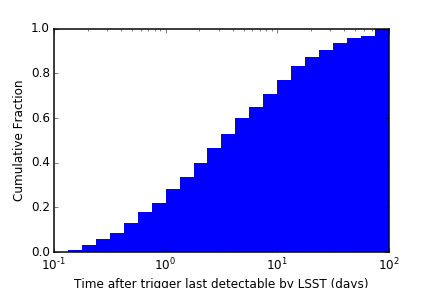
\includegraphics[width=0.6\textwidth]{figs/transients/afterglow_cdf.png}
}
\caption{ Cumulative fraction of GRB on-axis afterglows fainter than
magnitude 24.7 at a given time after the burst. We use an $\alpha=1$
decay with no jet breaks and the brightness parameters of
\citet{2011PASP..123.1034J}. }
\label{fig:afterglow_visibility}
\end{figure}

Thanks to LSST's depth, GRBs can be visible for weeks (Figure
\ref{fig:afterglow_visibility}).  Accordingly,
modest enhancements to the intra- and inter-night revisit rate with
single-filter rolling cadences should substantially improve LSST's
discovery and characterization of relativistic explosions.


% ====================================================================

\navigationbar
